\chapter{Digitaltechnik}
\textbf{Digital:} kann nur bestimmte (diskrete) Werte annehmen (z.B. 0/1, TRUE/FALSE; Digitaluhr 08:35 $\rightarrow$ 08:26 $\rightarrow$ 08:37)

\textbf{Analog:} kann beliebige (kontinuierliche) Werte annehmen (Temperaturmesswerte: 38.089°C, 40.05°C).

Aufgabe: Schaltung, mit zwei Schaltern, mit denen man Licht aus- und einschalten kann
\begin{center}	
\begin{tabular}{cc}
	\begin{circuitikz}[scale=1]
		\draw
		(1,0) node[spdt] (Sw1) {}		
		(2,0) node[spdt, xscale=-1] (Sw2) {}
		
		(Sw1.out 1) to (Sw2.out 1)
		(Sw1.out 2) to (Sw2.out 2)
		
		(0,0) to (Sw1.in)
		(Sw2.in) to (3,0)
		to (3,-1)
		to[lamp] (0,-1)
		
		(0,0) to[battery1] (0,-1)
		;
	\end{circuitikz}
	&
	\begin{tabular}{c|c||c}
		S1 & S2 & L \\
		\hline
		0 & 0 & 1 \\
		0 & 1 & 0 \\
		1 & 0 & 0 \\
		1 & 1 & 0 \\
	\end{tabular}
\end{tabular}
\end{center}	

\textbf{Allgemein}
\begin{itemize}
	\item mehrere Eingänge (a, b, c, d,...) (Schalter)
	\item einen Ausgang (x) (Lampe)
\end{itemize}

\section{Boolsche Algebra}
\textbf{Grundrechenwege} \\
\begin{tabular}{ccc}
	$\bullet$ UND (konjunktion) & \begin{tabular}{c|c||c}
		a & b & a $\land$ b \\
		\hline
		0 & 0 & 0 \\
		0 & 1 & 0 \\
		1 & 0 & 0 \\
		1 & 1 & 1 \\
	\end{tabular} & circuit \\

	& & \\
	
	$\bullet$ ODER (disjunktion) & \begin{tabular}{c|c||c}
		a & b & a $\lor$ b \\
		\hline
		0 & 0 & 0 \\
		0 & 1 & 1 \\
		1 & 0 & 1 \\
		1 & 1 & 0 \\
	\end{tabular} & circuit \\

	& & \\

	$\bullet$ NICHT (disjunktion) & \begin{tabular}{c||c}
		a & $\lnot$a oder $\overline{\text{a}}$ \\
		\hline
		0 & 1  \\
		0 & 0  \\
	\end{tabular} & \\
\end{tabular}


$\text{x}_1$ = a $\land$ (b $\lor$ c) \\
$\text{z}^{\text{Anzahl der Variablen}}$ = $\text{2}^\text{3}$ = 8

\begin{tabular}{c|c|c||c||c}
	a & b & c & b $\lor$ c & $\text{x}_1$ \\
	\hline
	0 & 0 & 0 & 0 & 0\\
	1 & 0 & 0 & 0 & 0\\
	0 & 1 & 1 & 1 & 0\\
	1 & 1 & 1 & 1 & 1\\
	0 & 0 & 1 & 1 & 0\\
	1 & 0 & 1 & 1 & 1\\
	0 & 1 & 1 & 1 & 0\\
	1 & 1 & 1 & 1 & 1\\
\end{tabular}

$\text{x}_2$ = a $\land$ b $\land$ c $\land$ $\overline{\text{a}}$ \\

\begin{tabular}{c|c|c|c||c||c||c}
	a & b & c & $\land$a & a $\land$ b & a $\land$ b $\land$ c & $\text{x}_2$ \\
	\hline
	0 & 0 & 0 & 1 & 0 & 0 & 0 \\
	1 & 0 & 0 & 0 & 0 & 0 & 0 \\
	0 & 1 & 0 & 1 & 0 & 0 & 0 \\
	1 & 1 & 0 & 0 & 1 & 0 & 0 \\
	0 & 0 & 1 & 1 & 0 & 0 & 0 \\
	1 & 0 & 1 & 0 & 0 & 0 & 0 \\
	0 & 1 & 1 & 1 & 0 & 0 & 0 \\
	1 & 1 & 1 & 0 & 1 & 1 & 0 \\
\end{tabular}

$\text{x}_3$ = a $\land$ b $\land$ ($\overline{\text{a}}$ $\lor$ c) \\

\begin{tabular}{c|c|c|c||c||c||c}
	a & b & c & $\overline{\text{a}}$ & (a $\lor$ c) & a $\land$ b & $\text{x}_3$ \\
	\hline
	0 & 0 & 0 & 1 & 1 & 0 & 0 \\
	1 & 0 & 0 & 0 & 0 & 0 & 0 \\
	0 & 1 & 0 & 1 & 1 & 0 & 0 \\
	1 & 1 & 0 & 0 & 0 & 1 & 0 \\
	0 & 0 & 1 & 1 & 1 & 0 & 0 \\
	1 & 0 & 1 & 0 & 1 & 0 & 0 \\
	0 & 1 & 1 & 1 & 1 & 0 & 0 \\
	1 & 1 & 1 & 0 & 1 & 1 & 1 \\
\end{tabular} \\
$\text{x}_3$ = a $\land$ b $\land$ c 

\textbf{Rechenregeln} \\
\begin{itemize}
	\item Vorrangsregeln\\
	$\lnot$ \textgreater $\land$ \textgreater $\lor$
	\item Kommutativgesetz \\
	a $\land$ b = b $\land$ a \\
	a $\lor$ b = b $\lor$ a 
	\item Assoziativgesetz \\
	a $\land$ (b $\land$ c) =(a $\land$ b) $\land$ c \\
	a $\lor$ (b $\lor$ c) =(a $\lor$ b) $\lor$ c
	\item Distributivgesetz \\
	a $\land$ (b $\lor$ c) = (a $\land$ b) $\lor$ (a $\land$ c) \\
	a $\lor$ (b $\land$ c) = (a $\lor$ b) $\land$ (a $\lor$ c)
	\item De Morgan'sche Gesetz \\
	$\overline{\text{a}\land\text{b}}$ = $\overline{\text{a}} \lor \overline{\text{b}}$ \\
	$\overline{\text{a}\lor\text{b}}$ = $\overline{\text{a}} \land \overline{\text{b}}$ 
\end{itemize}

\begin{tabular}{c|c|c|c||c||c||c}
	a & b & $\lnot$a & $\lnot$b & a $\land$ b & $\overline{\text{a}\land\text{b}}$ & $\lnot$a $\lor$ $\lnot$b \\
	\hline
	0 & 0 & 1 & 1 & 0 & 1 & 1 \\
	1 & 0 & 0 & 1 & 0 & 1 & 1 \\
	0 & 1 & 1 & 0 & 0 & 1 & 1 \\
	1 & 1 & 0 & 0 & 1 & 0 & 0 \\
\end{tabular} \\

\textbf{Weitere Gesetzte} \\
\begin{tabular}{p{\dimexpr 0.33\linewidth-2\tabcolsep} p{\dimexpr 0.33\linewidth-2\tabcolsep} p{\dimexpr 0.33\linewidth-2\tabcolsep}} 
	a $\land$ a = a & a $\land$ 1 = a & a $\land$ 0 = 0 \\
	a $\lor$ a = a & a $\lor$ 1 = 1 & a $\land$ 0 = a \\
	a $\land$ $\overline{\text{a}}$ = 0 & a $\lor$ $\overline{\text{a}}$ = 1 & \\
	$\overline{\overline{\text{a}}}$ = a & & \\
\end{tabular} 

\textbf{Standartschaltungen} \\
\begin{tabular}{ccl}
	$\bullet$ NAND 
	&
	\begin{tabular}{c|c||c}
		a & b & $\overline{\text{a} \land \text{b}}$ \\
		\hline
		0 & 0 & 1 \\
		1 & 0 & 1 \\
		0 & 1 & 1 \\
		1 & 1 & 0 \\
	\end{tabular} 
	& \\
	
	& & \\
	
	$\bullet$ NOR 
	&
	\begin{tabular}{c|c||c}
		a & b & $\overline{\text{a} \lor \text{b}}$ \\
		\hline
		0 & 0 & 1 \\
		1 & 0 & 0 \\
		0 & 1 & 0 \\
		1 & 1 & 0 \\
	\end{tabular} 
	& \\
	
	& & \\

	$\bullet$ Implikation 
	&
	\begin{tabular}{c|c||c}
		a & b & a $\rightarrow$ b \\
		\hline
		0 & 0 & 1 \\
		1 & 0 & 1 \\
		0 & 1 & 0 \\
		1 & 1 & 1 \\
	\end{tabular} 
	& a $\rightarrow$ b = $\overline{\text{a}} \lor \text{b}$ \\
	
		& & \\
	
	$\bullet$ Äquivalenz 
	&
	\begin{tabular}{c|c||c}
		a & b & a $\leftrightarrow$ b \\
		\hline
		0 & 0 & 1 \\
		1 & 0 & 0 \\
		0 & 1 & 0 \\
		1 & 1 & 1 \\
	\end{tabular} 
	& a $\leftrightarrow$ b = a $\rightarrow$ b $\land$ a $\rightarrow$ b = ($\overline{\text{a}}$ $\lor$ b) $\land$ ($\overline{\text{b}}$ $\lor$ a)\\
	
		& & \\
	
	$\bullet$ XOR 
	&
	\begin{tabular}{c|c||c}
		a & b & a $\oplus$ b \\
		\hline
		0 & 0 & 0 \\
		1 & 0 & 1 \\
		0 & 1 & 1 \\
		1 & 1 & 0 \\
	\end{tabular} 
	& a $\oplus$ b = a $\Leftrightarrow$ b \\
	
\end{tabular}

rechnungen bsps

\textbf{Normalformen} \\
\begin{tabular}{cc|c||c}
	  &a & b & x \\
	\hline
	1) & \text{\textcolor{red}{0}} & \text{\textcolor{red}{0}} & \text{\textcolor{red}{1}} \\
	2) & \text{\textcolor{OliveGreen}{1}} & \text{\textcolor{OliveGreen}{0}} & \text{\textcolor{OliveGreen}{0}} \\
	3) & \text{\textcolor{OliveGreen}{0}} & \text{\textcolor{OliveGreen}{1}} & \text{\textcolor{OliveGreen}{0}} \\
	4) & \text{\textcolor{red}{1}} & \text{\textcolor{red}{1}} & \text{\textcolor{red}{1}} \\
\end{tabular} \\
$\text{x}_{\text{\textcolor{red}{DNF}}}$ = ($\overline{\text{a}}$ $\land$ $\overline{\text{b}}$) $\lor$ (a $\land$ b) \\
\text{\textcolor{white}{-------------}} 1) \text{\textcolor{white}{----------}} 2)

$\text{x}_{\text{\textcolor{OliveGreen}{KNF}}}$ = (a $\lor$ $\overline{\text{b}}$) $\land$ ($\overline{\text{a}}$ $\lor$ b) \\
\text{\textcolor{white}{-------------}} 3) \text{\textcolor{white}{----------}} 4)

Aus einer Wahrheitstabelle mit beliebig vielen Eingängen und einem Ausgang kann immer eine Schaltung in DNF oder KNF angegeben werden.
\begin{itemize}
	\item DNF = Disjunktiv Normal Form (oder $\lor$)
	\item KNF = Konjunktiv Normal Form (oder $\land$)
\end{itemize}
Bei der DNF suchen wir jene Ausgänge, die '1' sind und verknüpfen die Eingänge mit einem '$\land$' wenn der Eingang '0' ist und verneinen sie. \\
Bei der KNF suchen wir jene Ausgänge die '0' sind und verknüpfen die Eingänge mit einem '$\lor$' wenn der Eingang '1' ist und verneinen sie.

wasserstand bsp...

\subsection{KV-Diagramme}
KV ... Karnaugh-Veitch \\

Pumpe x: 
\begin{tabular}{c|c|c|c|c}
	& \makecell{b = 0\\c = 0} & \makecell{b = 0\\c = 1} & \makecell{b = 1\\c = 1} & \makecell{b = 1\\c = 0} \\
	\hline
	a = 0 & 0 & 1 & 1 & 1 \\
	\hline
	a = 1 & 0 & 1 & 1 & 1 \\
\end{tabular} \\
x = c $\lor$ b \\

Pumpe y: 
\begin{tabular}{c|c|c|c|c}
	& \makecell{b = 0\\c = 0} & \makecell{b = 0\\c = 1} & \makecell{b = 1\\c = 1} & \makecell{b = 1\\c = 0} \\
	\hline
	a = 0 & 0 & 1 & 1 & 1 \\
	\hline
	a = 1 & 1 & 1 & 1 & 0 \\
\end{tabular} \\
y = c $\lor$ (a $\land$ $\overline{\text{b}}$) $\lor$ ($\overline{\text{a}}$ $\land$ b) \\

Pumpe z: 
\begin{tabular}{c|c|c|c|c}
	& \makecell{b = 0\\c = 0} & \makecell{b = 0\\c = 1} & \makecell{b = 1\\c = 1} & \makecell{b = 1\\c = 0} \\
	\hline
	a = 0 & 0 & 1 & 1 & 1 \\
	\hline
	a = 1 & 0 & 1 & 0 & 0 \\
\end{tabular} \\
z = ($\overline{\text{b}}$ $\land$ c) $\lor$ (b $\land$ $\overline{\text{a}}$) \\

Schaltplan: \\
%\begin{center}
%  \begin{circuitikz}
%		\ctikzset{logic ports = european}
%		\draw
%		(2,3) node[and port] (and1) {}
%		(2,2) node[and port] (and2) {}
%		(2,1) node[or port] (or1) {}
%		(2,0) node[and port] (and3) {}
%		
%		(5,2.5) node[or port] (or2) {}
%		(6,0) node[or port] (or3) {}
%				
%		(and1.in 1) node[left=.5cm](a0) {a}
%		(a0) -| (and1.in 1)
%				
%		(or1.in 1) node[left=.5cm](b0) {b}
%		(b0) -| (or1.in 1)
%		
%		(or1.in 2) node[left=.5cm](c0) {c}
%		(c0) -| (or1.in 2)
%		
%		(and1.out) -- ++(0.5,0) coordinate (And1out)
%		(or3.in 1) -- ++ (-0.5,0) -| (And1out)
%		(And1out) -| (or2.in 1)
%
%		(and2.out) -| (or2.in 2)
%
%		(and1.in 2) -- ++ (-0.25,0) coordinate (And1in2) 
%		(and2.in 1) -- ++ (-0.25,0) coordinate (And2in1)
%		(And2in1) -| (And1in2)
%		
%		(and3.in 1) -- ++(-0.25,0) coordinate (And3in1)
%		(And2in1) -| (And3in1)
%		
%		(or1.out) -- ++(2,0) node[right=.1cm]{x}
%		
%		(or1.in 2) -| (and2.in 2)
%		
%		;
%		% TODO: put o for NOT to some logic gates
%	\end{circuitikz}
%\end{center}

\begin{figure}[H]
	\centering
	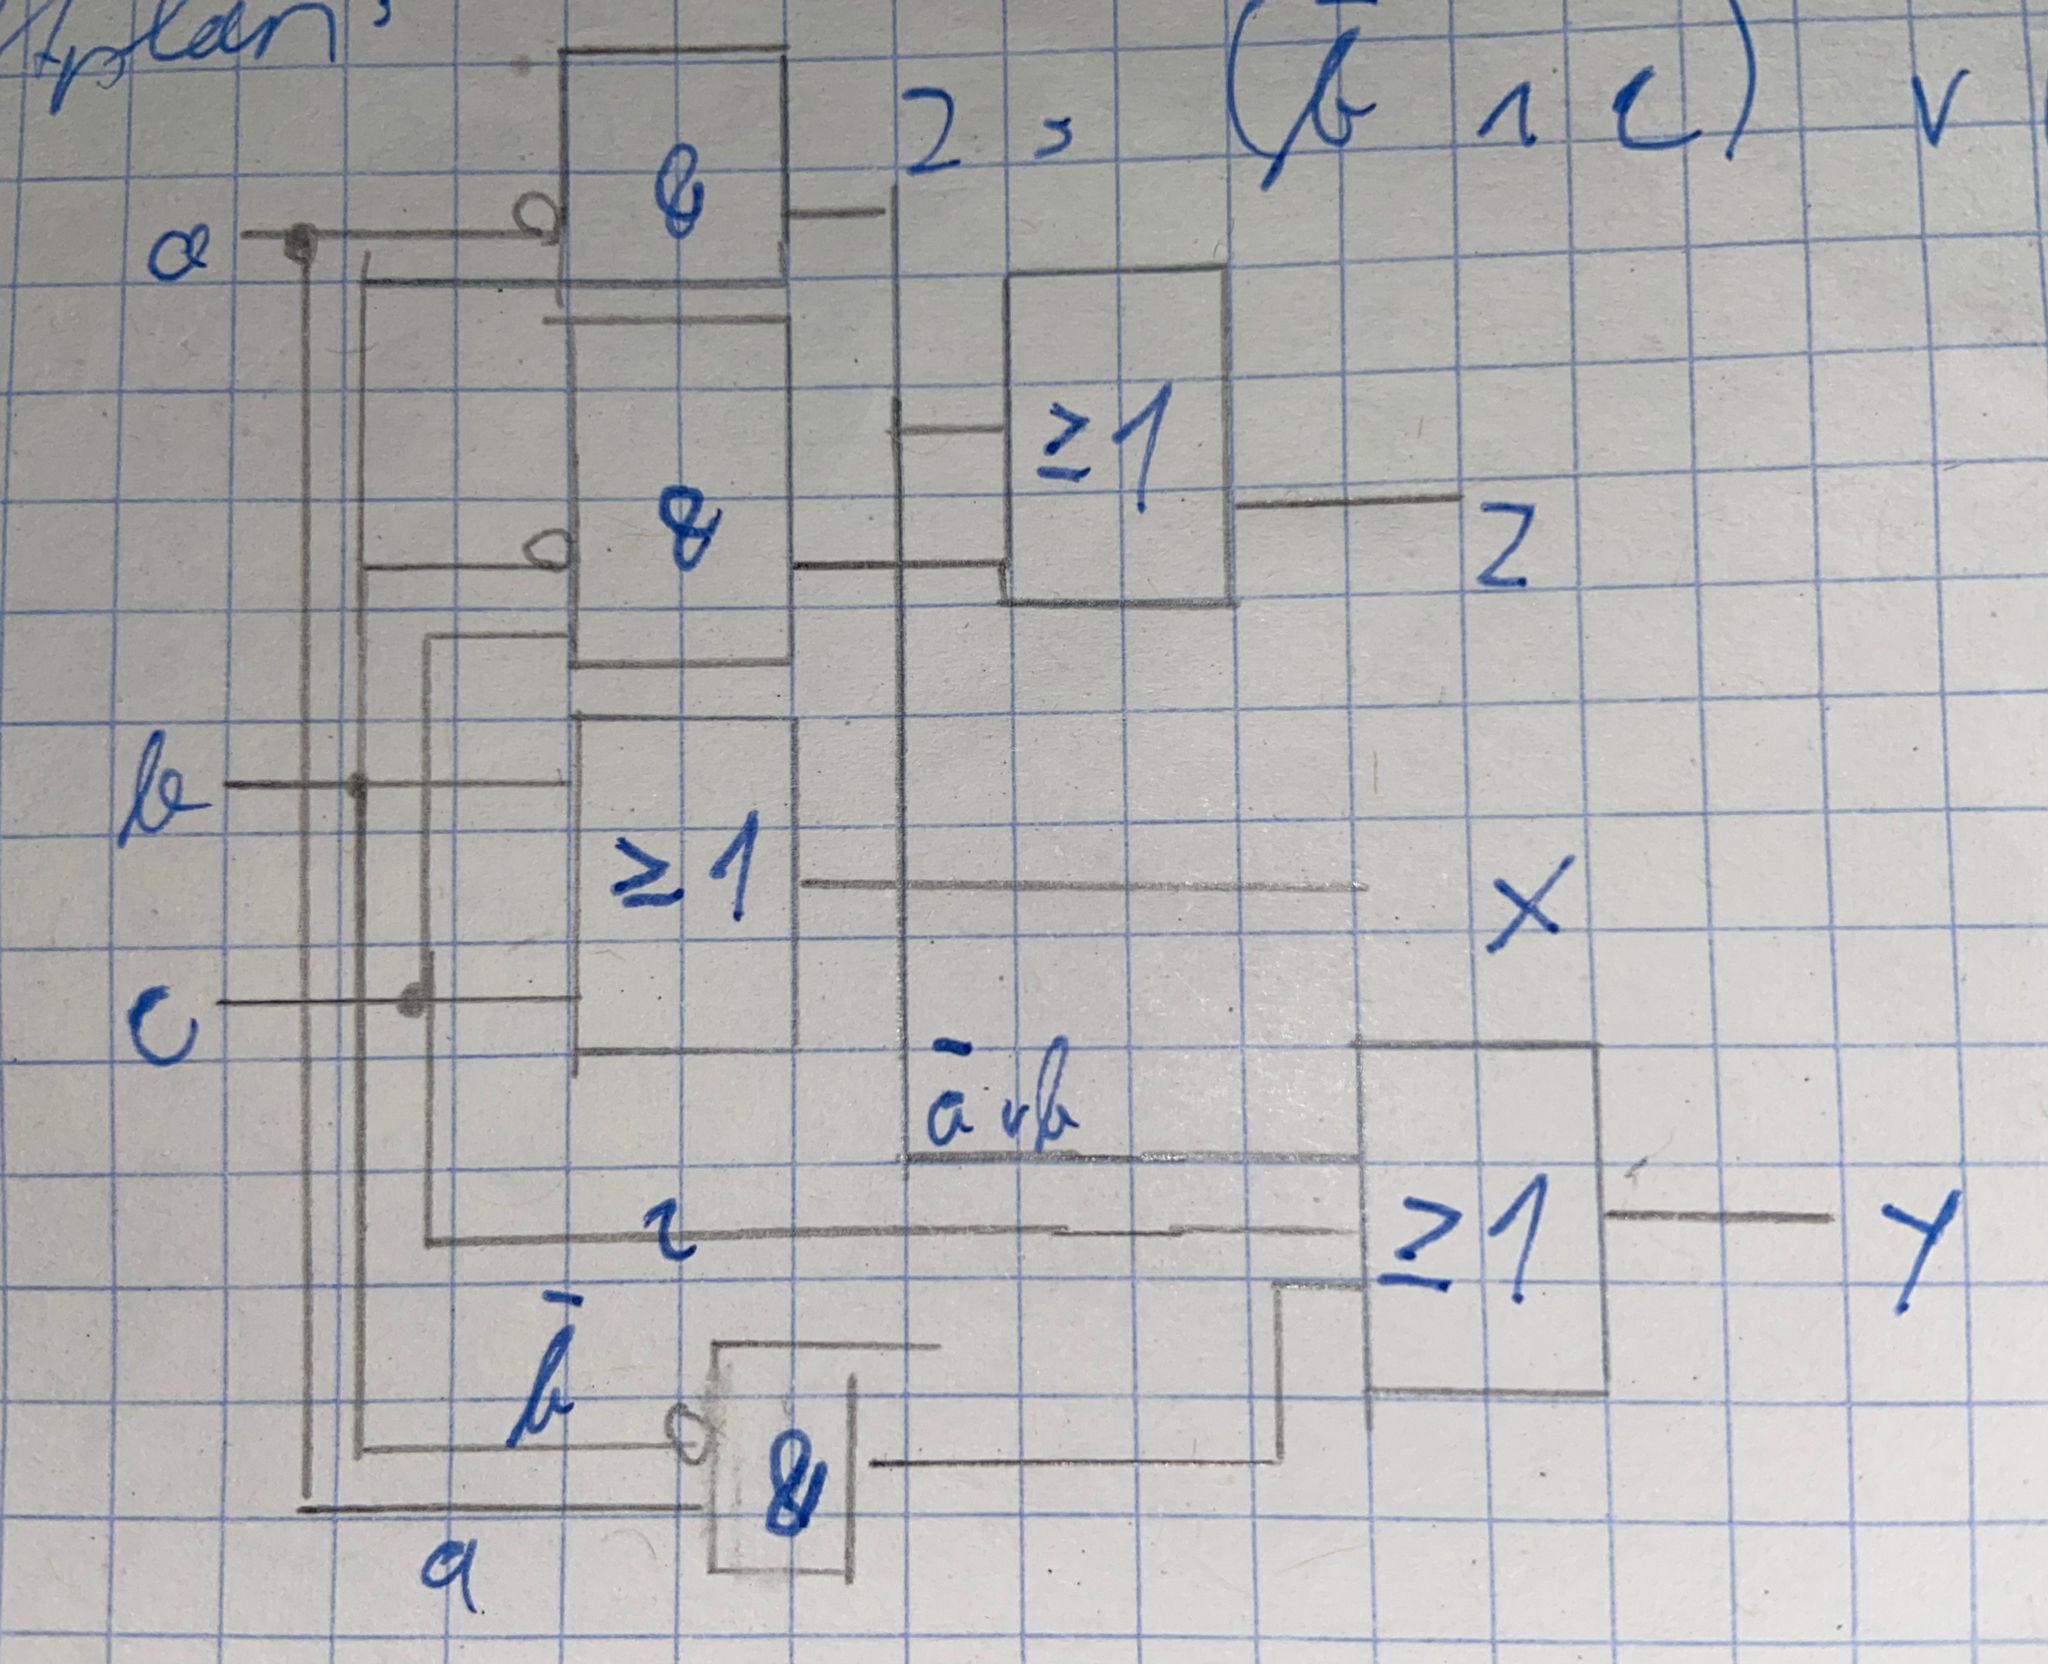
\includegraphics[width=0.8\linewidth]{figures/wasserschaltung.jpeg}
	\caption{Wasserpumpe Schaltung}
\end{figure}

\begin{tabular}{c|c|c||c|c}
	a & b & c & x & y \\
	\hline
	0 & 0 & 0 & 1 & 0 \\
	0 & 0 & 1 & 0 & 1 \\
	0 & 1 & 0 & 1 & 0 \\
	0 & 1 & 1 & 0 & 0 \\
	1 & 0 & 0 & 0 & 1 \\
	1 & 0 & 1 & 0 & 0 \\
	1 & 1 & 0 & 1 & 0 \\
	1 & 1 & 1 & 1 & 0 \\
\end{tabular}

$\text{x}_{\text{KNF}}$ = (a $\lor$ b $\lor$ $\overline{\text{c}}$) $\land$ (a $\lor$ $\overline{\text{b}}$ $\lor$ $\overline{\text{c}}$) $\land$ ($\overline{\text{a}}$ $\lor$ b $\lor$ c) $\land$ ($\overline{\text{a}}$ $\lor$ b $\lor$ $\overline{\text{c}}$) \\
$\text{x}_{\text{DNF}}$ = ($\overline{\text{a}}$ $\land$ $\overline{\text{b}}$ $\land$ $\overline{\text{c}}$) $\lor$ ($\overline{\text{a}}$ $\land$ b $\land$ $\overline{\text{c}}$) $\lor$ (a $\land$ b $\land$ $\overline{\text{c}}$) $\lor$ (a $\land$ b $\land$ c) \\

$\text{y}_{\text{KNF}}$ = (a $\lor$ b $\lor$ c) $\land$ (a $\lor$ $\overline{\text{b}}$ $\lor$ c) $\land$ (a $\lor$ $\overline{\text{b}}$ $\lor$ $\overline{\text{c}}$) $\land$ ($\overline{\text{a}}$ $\lor$ b $\lor$ $\overline{\text{c}}$) $\land$ ($\overline{\text{a}}$ $\lor$ $\overline{\text{b}}$ $\lor$ $\overline{\text{c}}$) \\
$\text{y}_{\text{DNF}}$ = ($\overline{\text{a}}$ $\land$ $\overline{\text{b}}$ $\land$ c) $\lor$ (a $\land$ $\overline{\text{b}}$ $\land$ $\overline{\text{c}}$) \\

\begin{tabular}{c|c|c|c|c}
	& \makecell{b = 0\\c = 0} & \makecell{b = 0\\c = 1} & \makecell{b = 1\\c = 1} & \makecell{b = 1\\c = 0} \\
	\hline
	a = 0 & 100 & 001 & 011 & 010 \\
	\hline
	a = 1 & 100 & 101 & 111 & 110 \\
\end{tabular}

(a $\land$ b) $\lor$ (a $\land$ b) \\

\begin{tabular}{c|c|c|c|c}
	x & \makecell{b = 0\\c = 0} & \makecell{b = 0\\c = 1} & \makecell{b = 1\\c = 1} & \makecell{b = 1\\c = 0} \\
	\hline
	a = 0 & 1 & 0 & 1 & 1 \\
	\hline
	a = 1 & 1 & 0 & 0 & 1 \\
\end{tabular}

x = $\overline{\text{c}}$ $\lor$ ($\overline{\text{a}}$ $\land$ b)

\subsection{KV-Diagramme mit 'Don't Care'}




